% Intended LaTeX compiler: pdflatex
\documentclass[conference, 10pt, final]{IEEEtran}
\usepackage[utf8]{inputenc}
\usepackage[T1]{fontenc}
\usepackage{graphicx}
\usepackage{longtable}
\usepackage{wrapfig}
\usepackage{rotating}
\usepackage[normalem]{ulem}
\usepackage{amsmath}
\usepackage{amssymb}
\usepackage{capt-of}
\usepackage{hyperref}
\usepackage[T1]{fontenc}
\usepackage{breakurl}
\usepackage{xspace}
\usepackage{listings}
\usepackage[font=footnotesize]{subfig}
\newcommand{\prettysmall}{\fontsize{4}{6}\selectfont}
\newcommand{\pstwo}{\fontsize{8}{8}\selectfont}
\usepackage{color,colortbl,xcolor}
\definecolor{dgeqrtC}{HTML}{e41a1c}
\definecolor{dlarfbC}{HTML}{377eb8}
\definecolor{dtpqrtC}{HTML}{4daf4a}
\definecolor{dtpmqrtC}{HTML}{984ea3}
\newcommand{\dgeqrtcolor}{red}
\newcommand{\dlarfbcolor}{blue}
\newcommand{\dtpqrtcolor}{green}
\newcommand{\dtpmqrtcolor}{purple}
\lstdefinestyle{customc}{morekeywords={DGEQRT },keywordstyle=\color{dgeqrtC},morekeywords=[2]{DLARFB},keywordstyle=[2]\color{dlarfbC},morekeywords=[3]{DTPQRT},keywordstyle=[3]\color{dtpqrtC},morekeywords=[4]{DTPMQRT},keywordstyle=[4]\color{dtpmqrtC}, numbers=left, breakatwhitespace=false,        breaklines=true,captionpos=b,keepspaces=true,numbersep=5pt,showspaces=false,showstringspaces=false,showtabs=false,tabsize=2}
\lstset{ basicstyle=\ttfamily\small, breaklines=true, columns=fullflexible,numbers=left,numberstyle=\tiny\color{gray}, xleftmargin=10pt,flexiblecolumns=false}
\usepackage{graphicx}
\usepackage{caption}
\usepackage{subcaption}
\usepackage{tikz}
\usetikzlibrary{automata,arrows,positioning,calc}
\usepackage{subfig}
\newcommand{\subfigureautorefname}{Figure} % allows autoref to find subimages.
\date{}
\title{LU-factor}
\hypersetup{
 pdfauthor={Otho José Sirtoli Marcondes, Lucas Mello Schnorr},
 pdftitle={LU-factor},
 pdfkeywords={},
 pdfsubject={},
 pdfcreator={Emacs 28.1 (Org mode 9.7.26)}, 
 pdflang={Portuges}}
\begin{document}


\title{Impact of Data Distribution and Schedulers for LU Factorization on Clusters}
% Let's keep the next title for the official post-WSPPD publication
% Visual Performance Analysis of Memory Operations in Heterogeneous Task-Based Applications}

\author{
\IEEEauthorblockN{Otho José Sirtoli Marcondes\IEEEauthorrefmark{1},
                  Lucas Mello Schnorr\IEEEauthorrefmark{1}}
\IEEEauthorblockN{\IEEEauthorrefmark{1} Institute of Informatics/PPGC/UFRGS, Porto Alegre, Brazil}
}

\maketitle

\newcommand{\kiter}{K Iteration}
\begin{abstract}
As the demand for more computational resources grows, the usage of clusters has become one of the main options to satisfy this need. In order to exploit these resources efficiently, the distribution of data between nodes must be considered as an important factor in application performance. This study aims to analyze the impact of the static block-cyclic data distribution and different dynamic schedulers of the linear algebra LU factorization on clusters. The analysis focuses on the execution time to explain how the application's behavior is influenced by the data distribution and scheduling strategy.

\end{abstract}
\section{Introduction}
\label{sec:orgf1ade28}
High-Performance Computing (HPC) systems, particularly computing clusters, are essential for solving large-scale scientific and engineering problems. These clusters consist of multiple interconnected nodes, each with its own processor units and memory. In order to maximize application performance on clusters, it is essential to consider both inter-node communication efficiency and workload balance across the computing nodes.

A crucial aspect of achieving efficient parallel performance is data partitioning, which determines how data is divided and distributed across the computing nodes. Among various strategies, static data partitioning is commonly used due to its simplicity and low runtime overhead. One of the examples of static data distribution is the block-cyclic (BC) distribution, a method that was popularized by the ScaLAPACK \cite{blackford1997scalapack} library.

This paper focuses on a scenario that combines static data partitioning with dynamic task scheduling. By leveraging task-based runtimes, we aim to dynamically schedule tasks at runtime while maintaining a static block layout of data. This approach enables better adaptability to runtime variations, such as load imbalance and communication delays, while preserving the advantages of a static data map.

As a case study, we explore the LU factorization, a fundamental operation in linear algebra widely used in scientific computing. We adopt a block cyclic distribution scheme for the input matrix, a method that balances the computational load and spreads data evenly across processes. Our goal is to evaluate how dynamic scheduling of tasks can improve the performance of LU factorization in clusters.

Throughout the development of this work, several challenges were encountered related to the use of MPI for executing applications across multiple nodes. These included: configuration challenges with Guix for package management across distributed nodes; issues related to the TCP interface in the MPI NewMadeleine implementation; and errors when using StarVZ \cite{pinto2021providing} visualization framework with the traces collected from the executions (still not resolved).

The paper is structured as follows. Section\textasciitilde{}\ref{sec:related} presents some related work on matrix distribution and modern task-based runtimes. Section\textasciitilde{}\ref{sec:methodology} details our methodology and explains how we conducted the experiments in our investigation. Section\textasciitilde{}\ref{sec:results} presents the experiments and their results. Section\textasciitilde{}\ref{sec:conclusion} concludes this work with some considerations.
\section{Related Work}
\label{sec:related}
\subsection{Matrix distribution}
\label{sec:org83081f3}
ScaLAPACK \cite{blackford1997scalapack} is the message passing version of LAPACK \cite{anderson1999lapack}, and also the standard library for linear algebra operations over parallel distributed platforms. In this paper, the LU factorization will be the focus, as its parallelization strategy is similar to others.

As shown in the Figure\textasciitilde{}\ref{fig:LU-factor}, the LU factorization of a given matrix \(A\) is defined as \(A=LU\), where \(L\) is a lower triangular matrix and \(U\) is an upper triangular matrix. The LU algorithm relies on three different LAPACK kernels: \verb|DGTRF-NOPIV|, \verb|DTRSM| and \verb|DGEMM|. This application has a tendency to be dominated by \verb|DGEMM| kernels when \(N\) is large, which makes it mandatory to have well distributed sub-matrixes between the nodes.

\begin{figure}[ht]
\centering
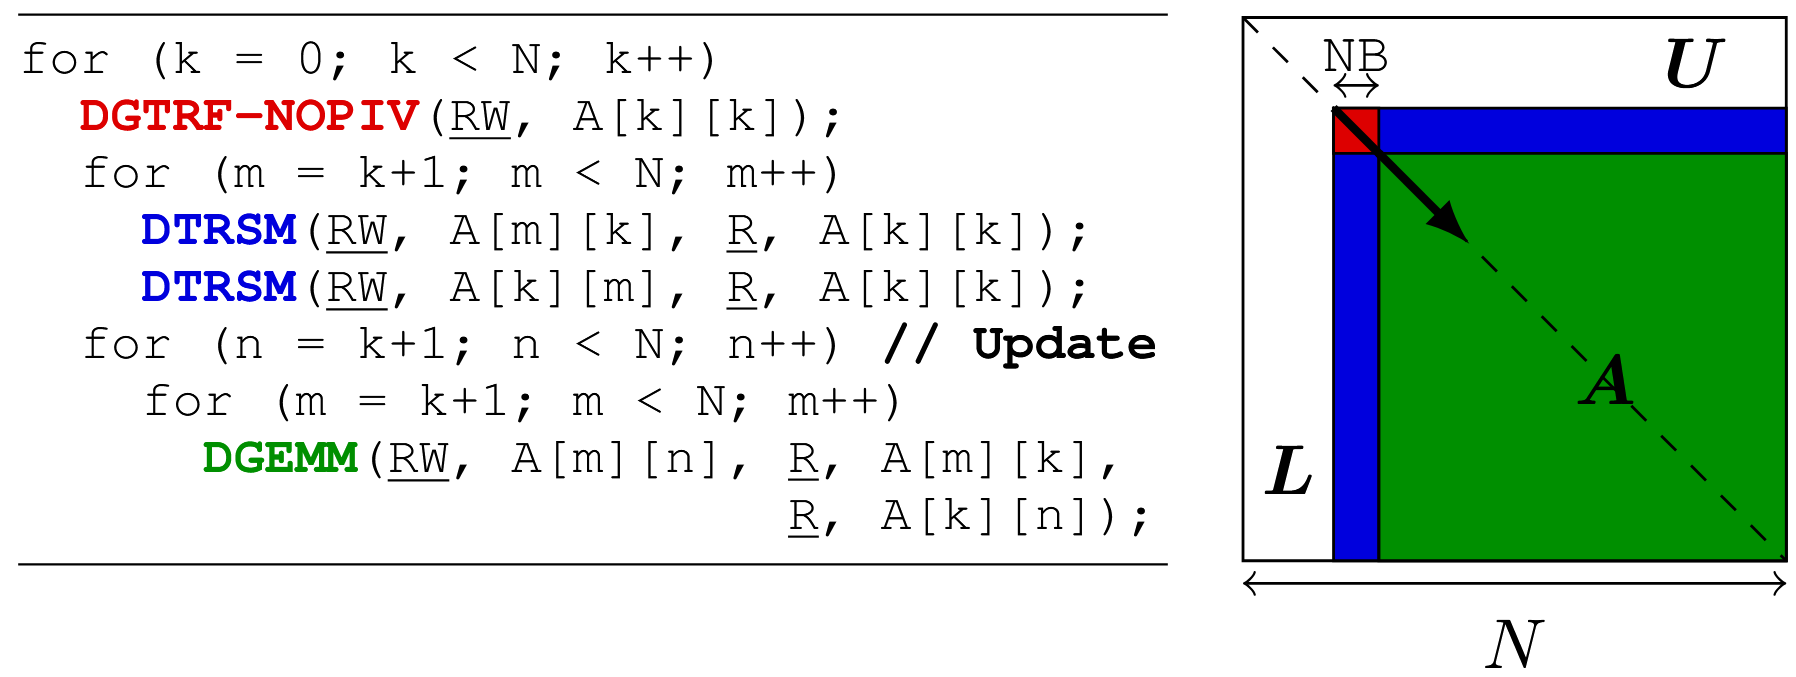
\includegraphics[width=.5\textwidth]{LU-factor.png}
\caption{The LU algorithm (left) without pivoting, and the regions of A updated at iteration k (right). \cite{nesi2020communication}}
\label{fig:LU-factor}
\end{figure}

The block cyclic distribution, popularized by the ScaLAPACK \cite{blackford1997scalapack} depends on the \(P x Q\) parameters and the number of available nodes. Based on the P value, the matrix will be partitioned differently across the nodes. In the Figure\textasciitilde{}\ref{fig:BC} we can visualize that while P is 1 (each panel show a PxQ distribution), there is only one node per row, as in reverse of the 8x1 distribution, where there is only one node per column. For the 2x4 and 4x2 cases, the distribution is interleaved.

\begin{figure}[ht]
\centering
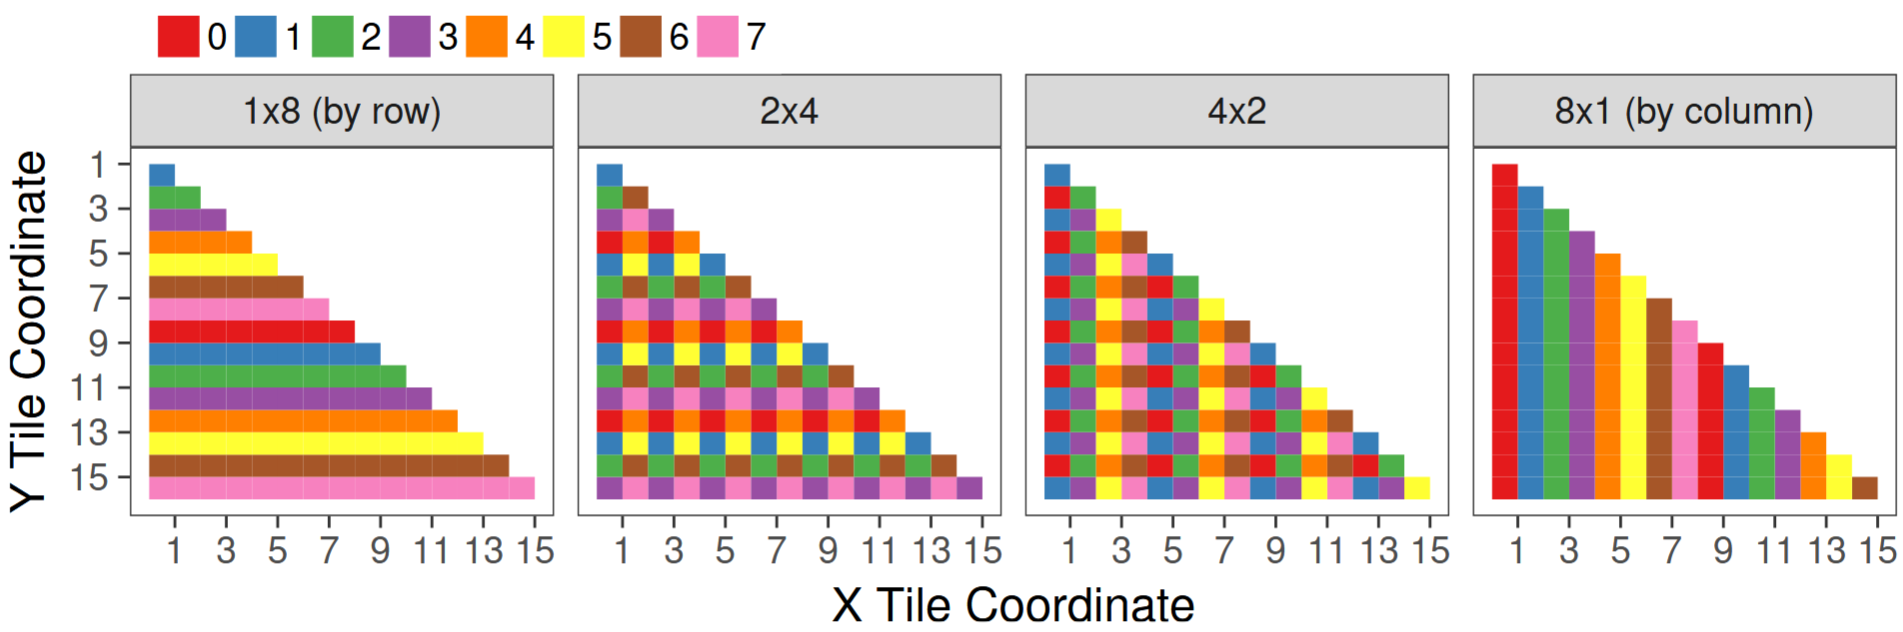
\includegraphics[width=.5\textwidth]{BC.png}
\caption{ Example of a block cyclic distribution across 8 nodes \cite{garcia2018visual}}
\label{fig:BC}
\end{figure}
\subsection{Task-based paradigm}
\label{sec:org8f285cd}

As the computers used in HPC environments became more complex, adapting and exploiting them to their full potential has become increasingly challenging. The task-based paradigm was designed to solve these new challenges. It relies on a DAG (Directed Acyclic Graph) to represent the relation between tasks and their dependencies (edges). The scheduler then can dynamically allocate these tasks during execution time, according to the dependencies of the graph and the scheduler heuristic \cite{faverge2023programming}. Chameleon \cite{agullo:inria-00547847}, as other linear algebra libraries such as DPLASMA \cite{bosilca2011flexible} are built on task-based runtimes, which allows them to efficiently exploit their computational resources of clusters. The scheduler heuristics studied in this work are the following:

\begin{itemize}
\item \verb|lws|: stands for locality work stealing. When a worker becomes idle, it steals a task from a neighboring worker;

\item \verb|random|: tasks are distributed randomly according the assumed worker overall performance;

\item \verb|dmda|: takes task execution performance models and data transfer time into account;

\item \verb|dmdas|: same as \verb|dmda|, but also take into account task priorities and data buffer availability on the target device.

\end{itemize}
\section{{\bfseries\sffamily TODO} Experimental Methodology}
\label{sec:methodology}
To enable execution on multiple nodes, we employed StarPU \cite{augonnet2009starpu}, which provides a variety of scheduling policies and built-in support for application tracing.

StarPU is a task-based runtime system for heterogeneous platforms, being multicore or multinode. The StarPU uses the Sequential Task-Flow (STF) \cite{kennedy2001optimizing}, where the tasks are sequentially submitted to the runtime that is responsible for their scheduling. Each task can have one implementation for a respective computational resource (CPU, GPU) called worker, and the scheduler must assign a task to one of the available workers during the program execution. To enable multi-node execution, the StarPU-MPI extension was used \cite{augonnet2012starpu}.

We utilized Chameleon \cite{agullo:inria-00547847} implementation of the LU factorization, with 64x64 block size for all experiments. This value was taken from a preliminary execution only varying the block size as shown in Figure\textasciitilde{}\ref{fig:timeBlocks}, that depicts different blocks dimensions and their respective execution times. It is possible to observe that the 64x64 block size had the best performance among the other values.

\begin{figure}[ht]
\centering
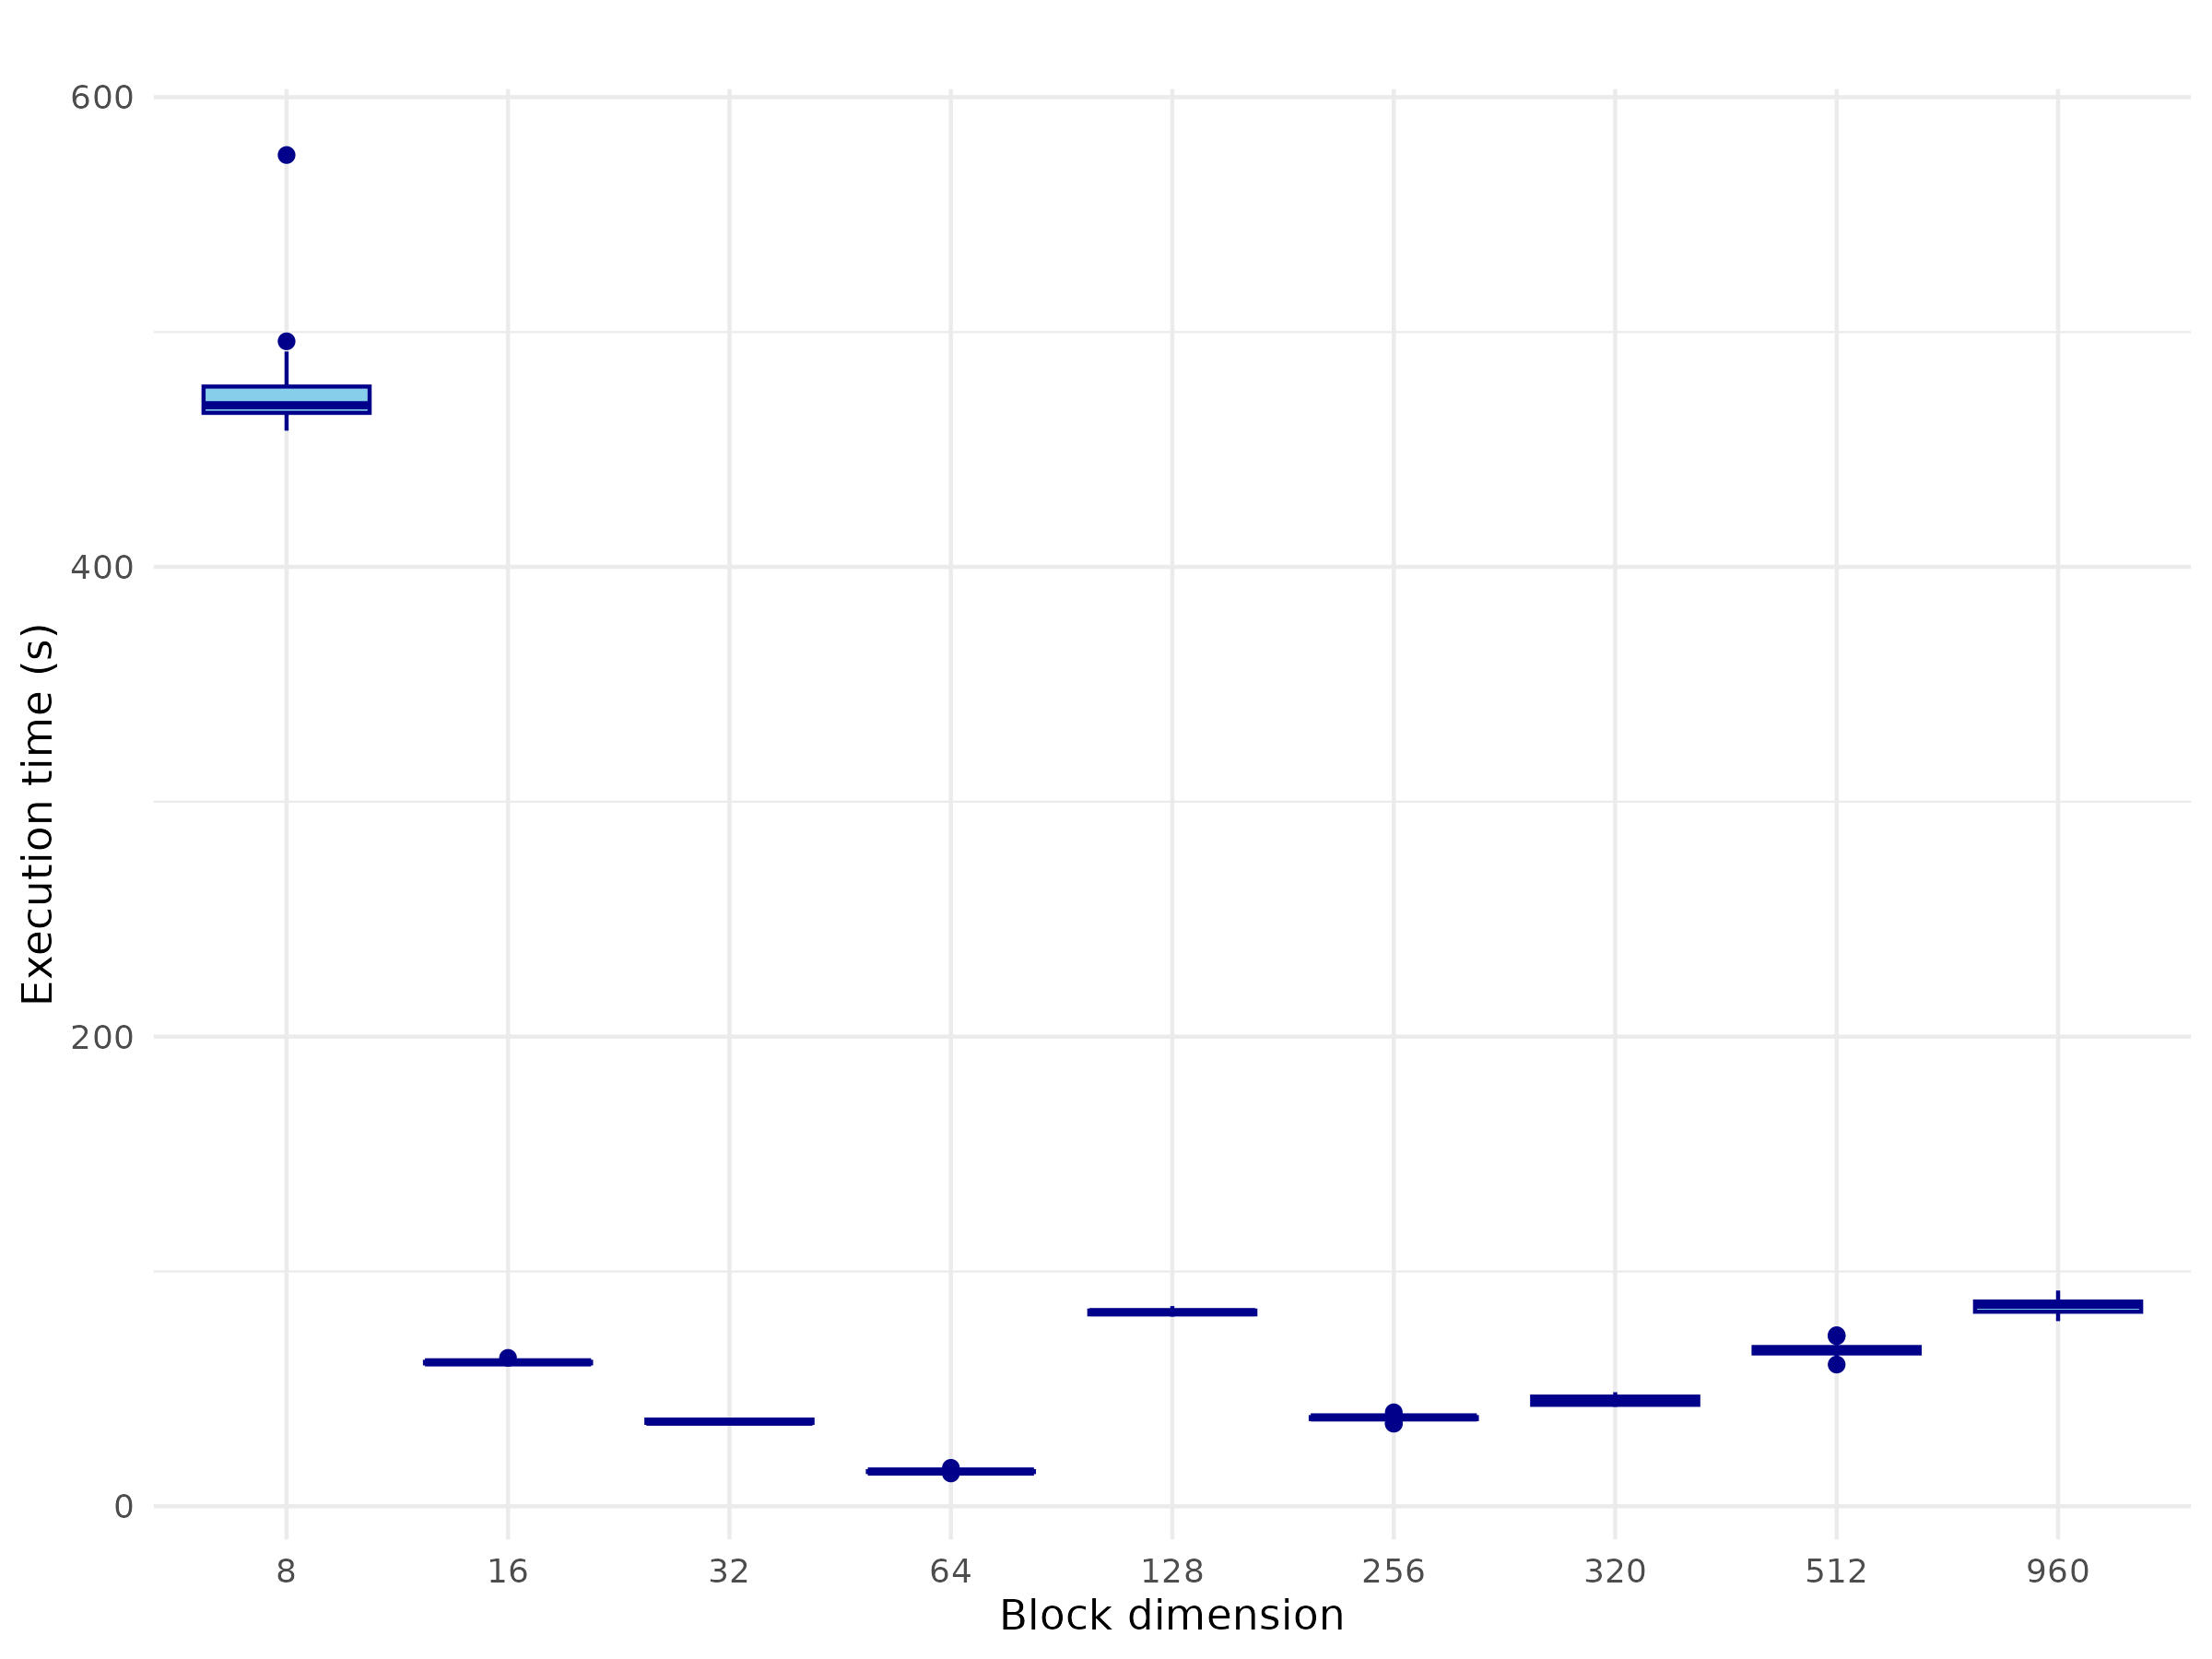
\includegraphics[width=0.5\textwidth]{boxplot_tempo_por_nb.png}
\caption{Execution times per block dimension}
\label{fig:timeBlocks}
\end{figure}

\% IMAGE OF BLOCK SIZE

The executions were performed in the PCAD from UFRGS using the \verb|Cei| partition. \verb|Cei| comprises six nodes, each one with two Intel Xeon Silver 4116 (24 cores/CPU). We used the 1.4.7 StarPU and 1.3.0 Chameleon version. We also used NewMadeleine \cite{aumage2007new} MPI implementation as OpenMPI \cite{gabriel2004open} presented significant idle times during the executions. The NewMadeleine version used was from commit \verb|6e1a64d0| from June 2025, which resolved a TCP interface issue that we reported. For the execution time evaluation, each execution was run 10 times and the standard deviation was lower than 5$\backslash$%.
\section{{\bfseries\sffamily TODO} Results}
\label{sec:results}
Figure\textasciitilde{}\ref{fig:timePQ} depicts four panels, aligned in the X dimension (time), each showing the execution time of a different scheduler (\verb|random|, \verb|lws|, \verb|dmdas|, \verb|dmda|) with a fixed PxQ configuration. The standard deviation is represented by the black error bars on each bar. We can see that the \verb|lws| and \verb|random| schedulers did not present much variation when changing the PxQ configuration. As for the \verb|dmdas| and \verb|dmda|, both of them showed significantly better performance when utilizing the \(P=2\) \(Q=3\) and \(P=3\) \(Q=2\) configurations.

\begin{figure}[ht]
\centering
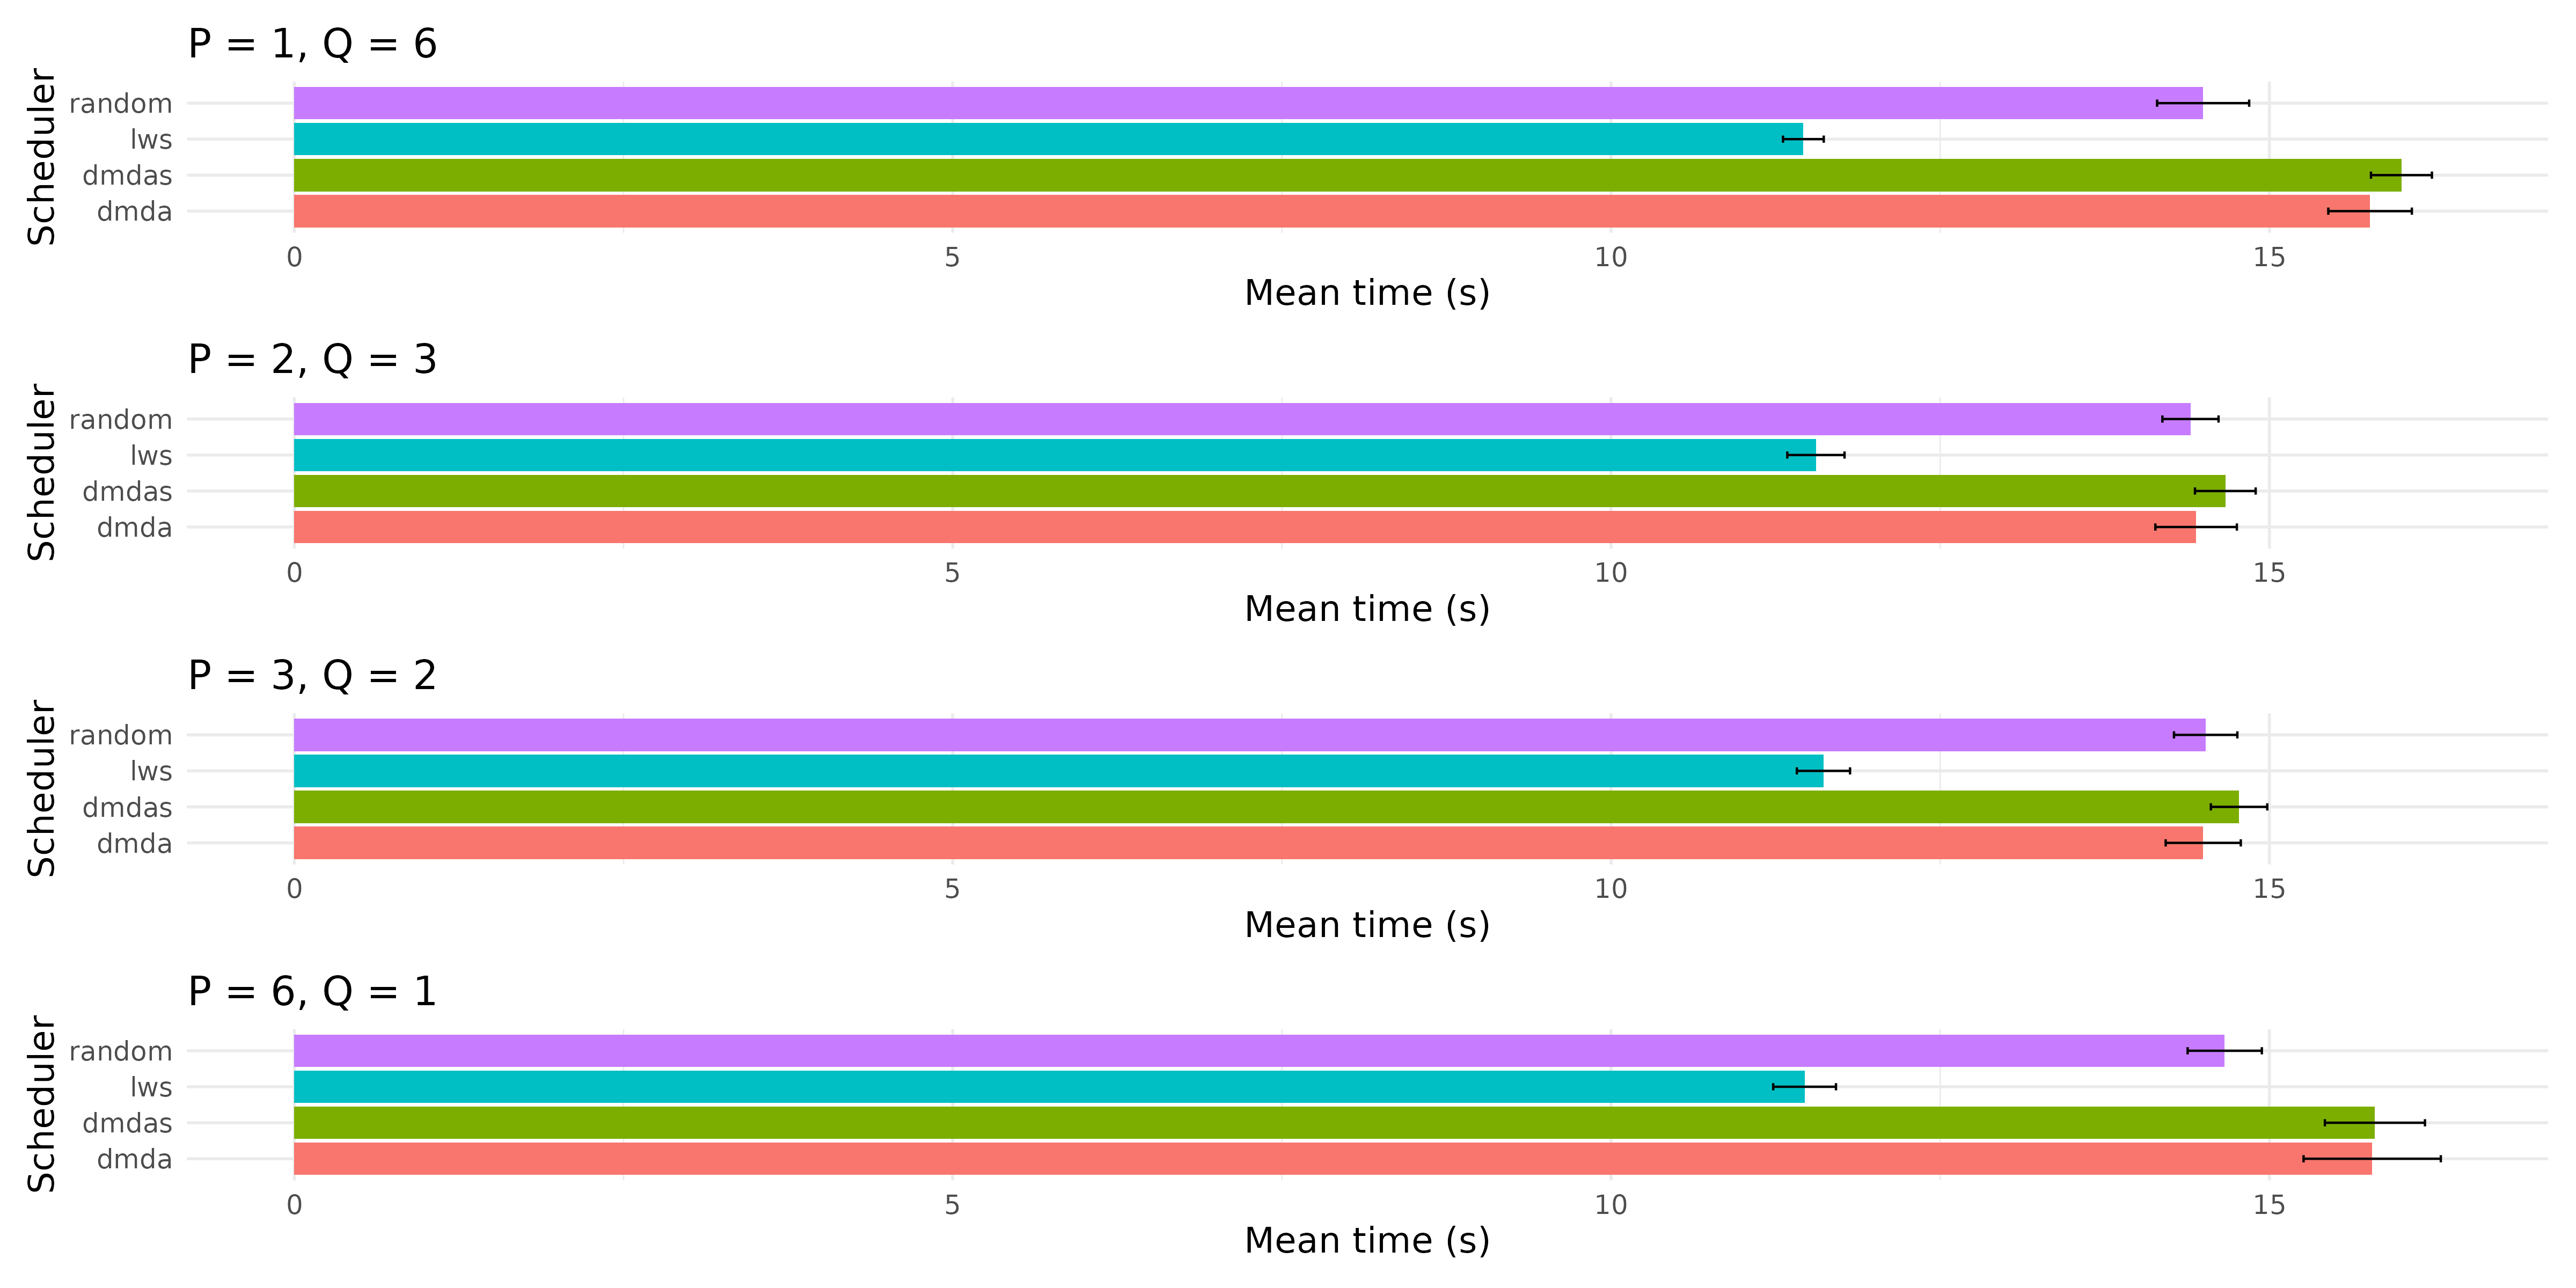
\includegraphics[width=0.5\textwidth]{tempo_medio_com_desvio_padrao_por_PQ.png}
\caption{Execution times based on the PxQ configuration}
\label{fig:timePQ}
\end{figure}

Figure\textasciitilde{}\ref{fig:timeSched} depicts four panels, aligned in the X dimension (time), each of them showing the execution time of a PxQ configuration with a fixed scheduler heuristic. The standard deviation is represented by the black error bars on each bar. We can see that the \verb|lws| scheduler had the best results among the schedulers fallowed by the \verb|random| scheduler. The \verb|dmda| and \verb|dmdas| had similar performance, with performance gains when P and Q are interleaved.

\begin{figure}[ht]
\centering
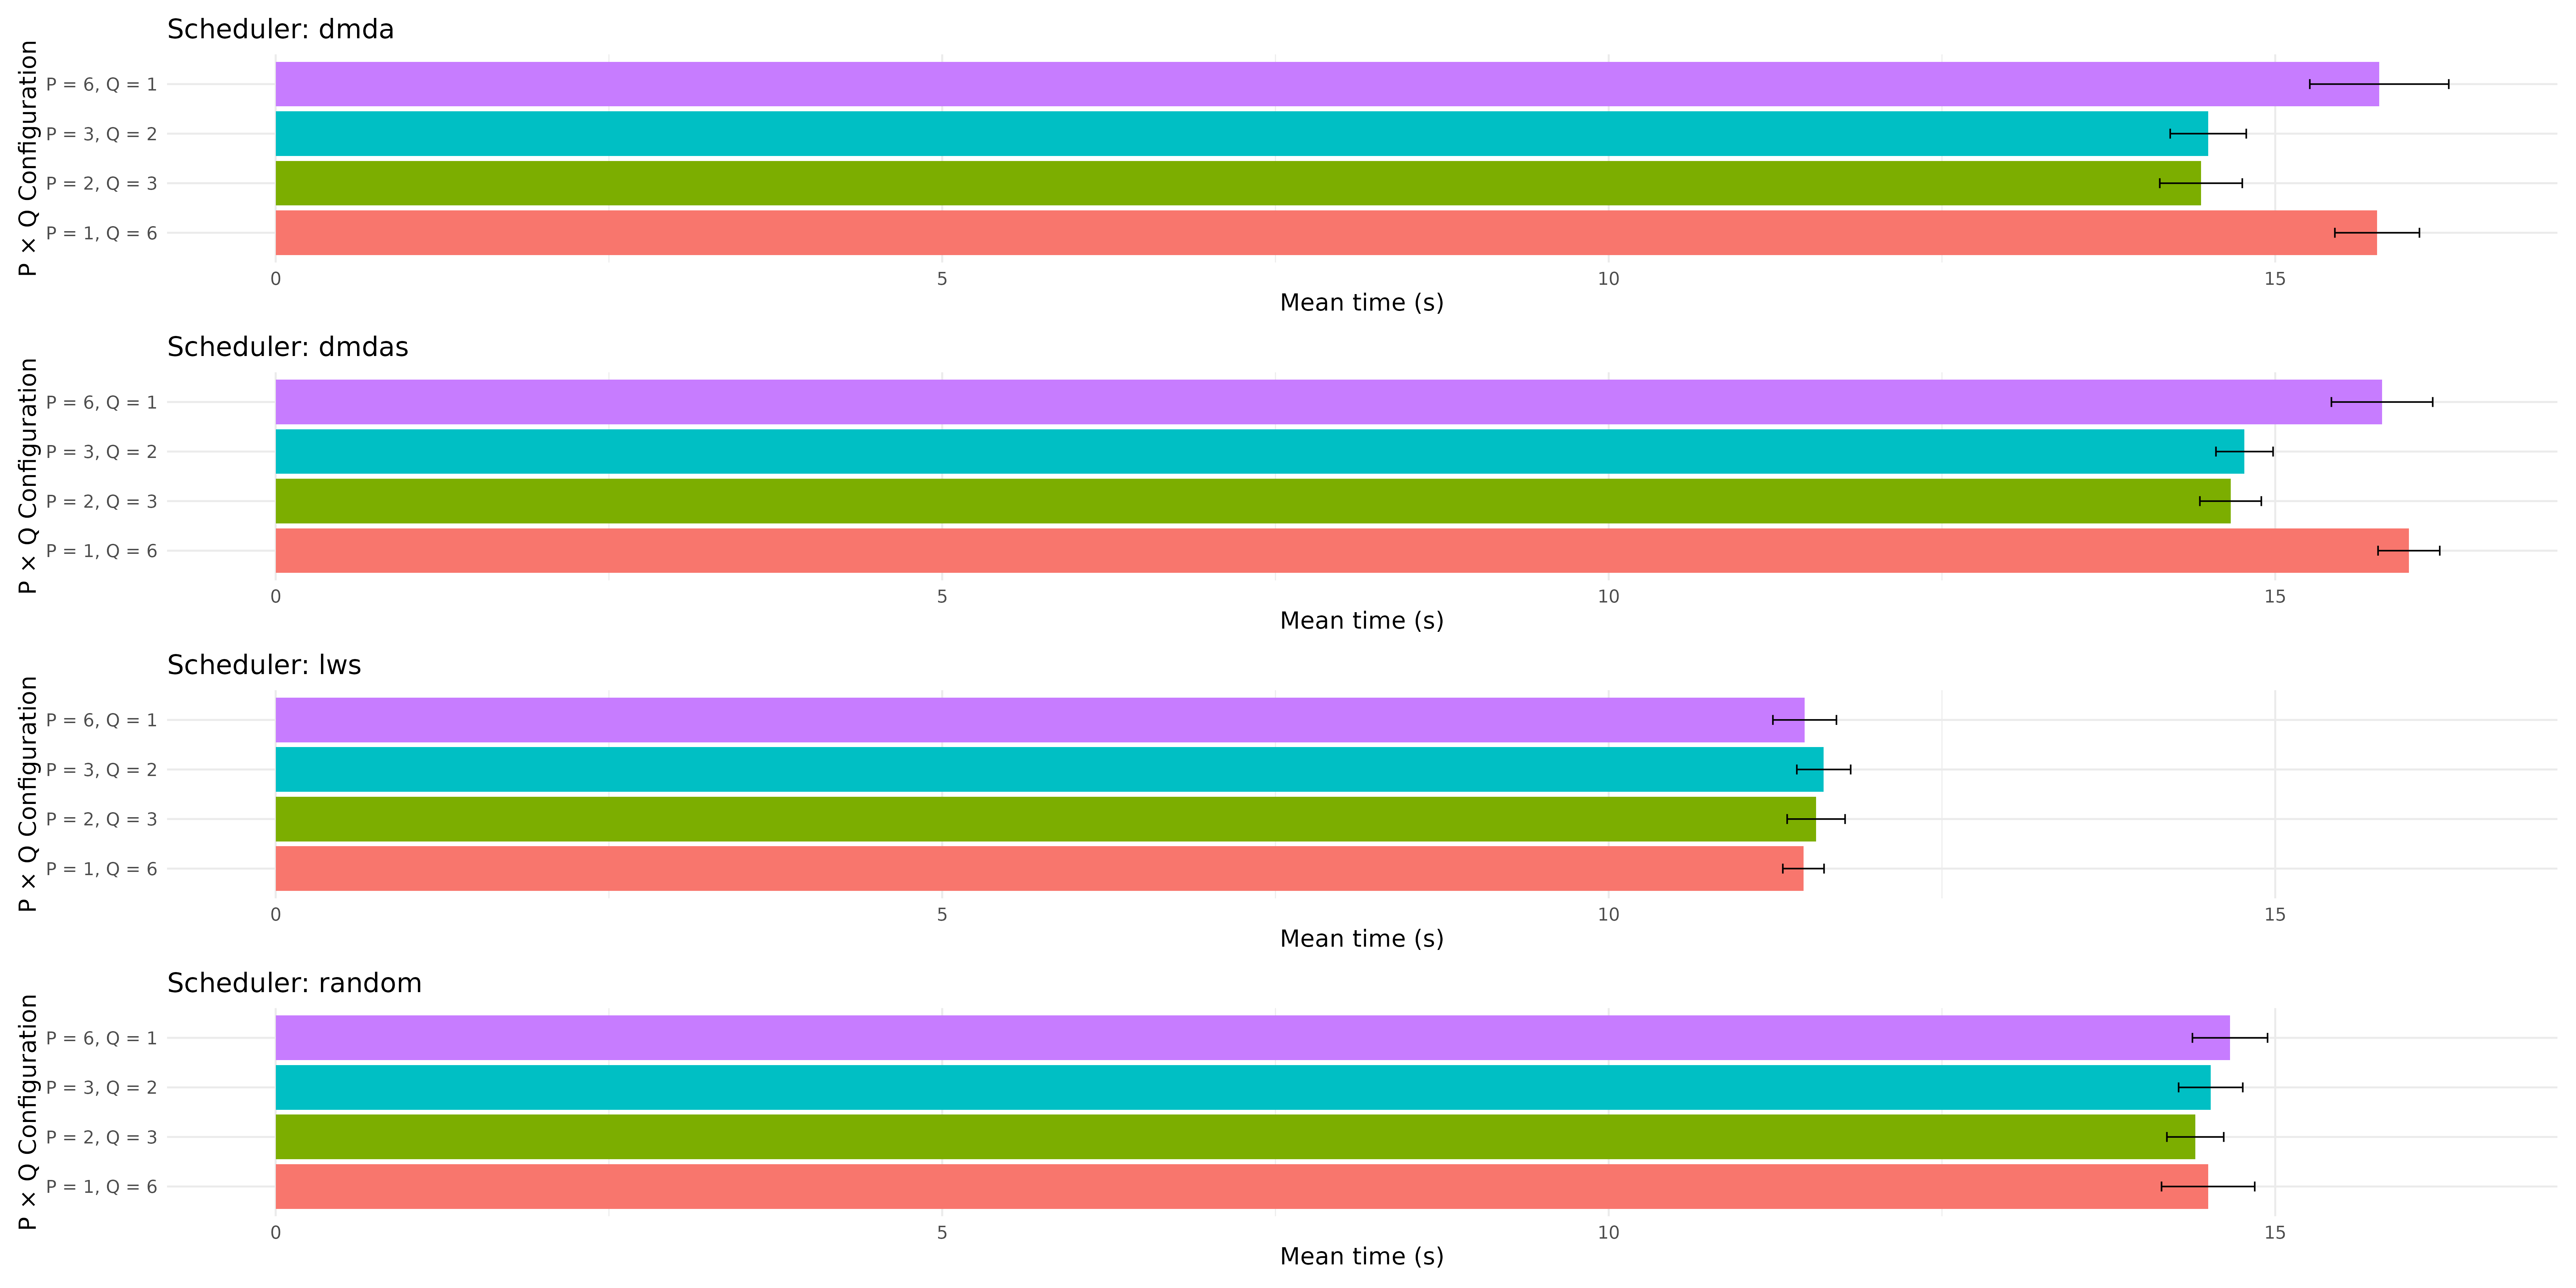
\includegraphics[width=0.5\textwidth]{tempo_medio_com_desvio_padrao_por_scheduler.png}
\caption{Execution times based on the scheduler heuristic}
\label{fig:timeSched}
\end{figure}
\section{{\bfseries\sffamily TODO} Conclusion}
\label{sec:conclusion}
The study examines the impact of data distribution using Block cyclic and also the impact of different scheduler heuristics in the context of task-based runtime in clusters. The linear algebra LU factorization application provided by Chameleon was used as a means to analyze how these configurations impact performance. The \verb|dmda| and \verb|dmdas| heuristics presented similar behavior in their execution times, showing performance gains when the P and Q were interleaved. The \verb|lws| heuristic presented the best results in terms of performance, although the P and Q parameters did not have significant impact in it. The \verb|random| heuristic also showed no significant impact on its performance based on the P and Q parameters.

The various issues encountered during the development of this work caused the executions utilizing NewMadeleine implementation of MPI were only conducted toward the end of the available time. Also, to build a stronger argument about why a given scheduler or distribution outperformed the others, the use of execution traces would be necessary. These traces would make possible to visualize the behavior of the application during its execution. As previously mentioned, there are still ongoing problems in the utilization of the FxT traces with the StarVZ framework. The next steps would consist of: resolve the issues preventing StarVZ usage and use SimGrid \cite{CASANOVA2025103125} to run simulations and scale the number of nodes.
\section*{Acknowledgements}

The experiments in this work used the PCAD infrastructure, \url{http://gppd-hpc.inf.ufrgs.br}, at INF/UFRGS.
\clearpage

\bibliographystyle{IEEEtran}
\bibliography{refs}
\end{document}
